% !BIB TS-program = biber
\RequirePackage[l2tabu,orthodox]{nag}
% TODO: decide if one-sided/two-sided
%\documentclass[headsepline,footsepline,footinclude=false,fontsize=11pt,paper=a4,listof=totoc,bibliography=totoc,BCOR=12mm,DIV=12]{scrbook} % two-sided
\documentclass[headsepline,footsepline,footinclude=false,oneside,fontsize=11pt,paper=a4,listof=totoc,bibliography=totoc]{scrbook} % one-sided
% TODO: change thesis information
\usepackage{graphicx}
\usepackage{tikz}
\usetikzlibrary{positioning}
\usetikzlibrary{calc,patterns}
\usetikzlibrary{shapes.geometric, arrows}
\tikzstyle{startstop} = [rectangle, rounded corners, minimum width=1cm, minimum height=1cm, text centered, draw=black]
\tikzstyle{process} = [rectangle, minimum width=1cm, minimum height=1cm, text centered, draw=black]
\tikzstyle{decision} = [diamond, minimum width=1cm, minimum height=1cm, text centered, draw=black]
\tikzstyle{arrow} = [thick,->,>=stealth]

\newcommand*{\getUniversity}{Technische Universität München}
\newcommand*{\getFaculty}{Informatics}
\newcommand*{\getDegree}{Informatics}
\newcommand*{\getSchool}{Computation, Information and Technology}
\newcommand*{\getTitle}{Tooling and Benchmarking of a Hardware-Agnostic Compilation Toolchain For Neutral-Atom Quantum Computers}
\newcommand*{\getTitleGer}{Tooling und Benchmarking einer hardwareunabhängigen Kompilierung Toolchain für Neutralatom-Quantencomputer}
\newcommand*{\getAuthor}{Emil Khusainov}
\newcommand*{\getDoctype}{Bachelor's Thesis}
\newcommand*{\getSupervisor}{Prof. Dr. Christian Mendl}
\newcommand*{\getAdvisor}{M.Sc. Yanbin Chen}
\newcommand*{\getKeywords}{keyword;another keyword;one more}
\newcommand*{\getSubmissionDate}{04.07.2035}
\newcommand*{\getSubmissionLocation}{Munich}

% TODO: change citation style in settings
\PassOptionsToPackage{table,svgnames,dvipsnames}{xcolor}

\usepackage[a-2u]{pdfx} % generate PDF/A: archival compliant, self-contained pdf
\usepackage[utf8]{inputenc}
\usepackage[T1]{fontenc}
\usepackage[sc]{mathpazo}
\usepackage[ngerman,american]{babel}
\usepackage[autostyle]{csquotes}
\usepackage[%
  backend=biber,
  url=true,
  style=numeric,
  maxnames=4,
  minnames=3,
  maxbibnames=99,
  giveninits,
  uniquename=init]{biblatex} % TODO: adapt citation style
\usepackage{graphicx}
\usepackage{scrhack} % necessary for listings package
\usepackage{listings}
\usepackage{lstautogobble}
\usepackage{tikz}
\usepackage{pgfplots}
\usepackage{pgfplotstable}
\usepackage{booktabs}
\usepackage[final]{microtype}
\usepackage{caption}
\usepackage[printonlyused]{acronym}
\usepackage{ifthen}


\hypersetup{hidelinks} % removes colored boxes around references and links

% for fachschaft_print.pdf
\makeatletter
\if@twoside
	\typeout{TUM-Dev LaTeX-Thesis-Template: twoside}
\else
	\typeout{TUM-Dev LaTeX-Thesis-Template: oneside}
\fi
\makeatother

\addto\extrasamerican{
	\def\lstnumberautorefname{Line}
	\def\chapterautorefname{Chapter}
	\def\sectionautorefname{Section}
	\def\subsectionautorefname{Subsection}
	\def\subsubsectionautorefname{Subsubsection}
}

\addto\extrasngerman{
	\def\lstnumberautorefname{Zeile}
}

% Themes
\ifthenelse{\equal{\detokenize{dark}}{\jobname}}{%
  % Dark theme
  \newcommand{\bg}{black} % background
  \newcommand{\fg}{white} % foreground
  \usepackage[pagecolor=\bg]{pagecolor}
  \color{\fg}
}{%
  % Light theme
  \newcommand{\bg}{white} % background
  \newcommand{\fg}{black} % foreground
}

\bibliography{bibliography}

\setkomafont{disposition}{\normalfont\bfseries} % use serif font for headings
\linespread{1.05} % adjust line spread for mathpazo font

% Add table of contents to PDF bookmarks
\BeforeTOCHead[toc]{{\cleardoublepage\pdfbookmark[0]{\contentsname}{toc}}}

% Define TUM corporate design colors
% Taken from http://portal.mytum.de/corporatedesign/index_print/vorlagen/index_farben
\definecolor{TUMBlue}{HTML}{0065BD}
\definecolor{TUMSecondaryBlue}{HTML}{005293}
\definecolor{TUMSecondaryBlue2}{HTML}{003359}
\definecolor{TUMBlack}{HTML}{000000}
\definecolor{TUMWhite}{HTML}{FFFFFF}
\definecolor{TUMDarkGray}{HTML}{333333}
\definecolor{TUMGray}{HTML}{808080}
\definecolor{TUMLightGray}{HTML}{CCCCC6}
\definecolor{TUMAccentGray}{HTML}{DAD7CB}
\definecolor{TUMAccentOrange}{HTML}{E37222}
\definecolor{TUMAccentGreen}{HTML}{A2AD00}
\definecolor{TUMAccentLightBlue}{HTML}{98C6EA}
\definecolor{TUMAccentBlue}{HTML}{64A0C8}

% Settings for pgfplots
\pgfplotsset{compat=newest}
\pgfplotsset{
  % For available color names, see http://www.latextemplates.com/svgnames-colors
  cycle list={TUMBlue\\TUMAccentOrange\\TUMAccentGreen\\TUMSecondaryBlue2\\TUMDarkGray\\},
}

% Settings for lstlistings
\lstset{%
  basicstyle=\ttfamily,
  columns=fullflexible,
  autogobble,
  keywordstyle=\bfseries\color{TUMBlue},
  stringstyle=\color{TUMAccentGreen},
  captionpos=b
}


\begin{document}

% Set page numbering to avoid "destination with the same identifier has been already used" warning for cover page.
% (see https://en.wikibooks.org/wiki/LaTeX/Hyperlinks#Problems_with_Links_and_Pages).
\pagenumbering{alph}
\begin{titlepage}
  % HACK for two-sided documents: ignore binding correction for cover page.
  % Adapted from Markus Kohm's KOMA-Script titlepage=firstiscover handling.
  % See http://mirrors.ctan.org/macros/latex/contrib/koma-script/scrkernel-title.dtx,
  % \maketitle macro.
  \oddsidemargin=\evensidemargin\relax
  \textwidth=\dimexpr\paperwidth-2\evensidemargin-2in\relax
  \hsize=\textwidth\relax

  \centering

  \IfFileExists{logos/tum-\fg.pdf}{%
    \includegraphics[height=20mm]{logos/tum-\fg.pdf}
  }{%
    \vspace*{20mm}
  }

  \vspace{5mm}
  {\huge\MakeUppercase{School of \getSchool{} --- \getFaculty{}} \par}

  \vspace{5mm}
  {\large\MakeUppercase{\getUniversity{}} \par}

  \vspace{15mm}
  {\Large \getDoctype{} in \getDegree{} \par}

  \vspace{10mm}
  {\huge\bfseries \getTitle{} \par}

  \vspace{10mm}
  {\LARGE \getAuthor{}}

  \IfFileExists{logos/faculty-\fg.pdf}{%
    \vfill{}
    \includegraphics[height=20mm]{logos/faculty-\fg.pdf}
  }{}
\end{titlepage}


\frontmatter{}

\begin{titlepage}
  \centering

  \IfFileExists{logos/tum-\fg.pdf}{%
    \includegraphics[height=20mm]{logos/tum-\fg.pdf}
  }{%
    \vspace*{8mm}
  }

  \vspace{5mm}
  {\huge\MakeUppercase{School of \getSchool{} --- \getFaculty{}} \par}

  \vspace{5mm}
  {\large\MakeUppercase{\getUniversity{}} \par}

  \vspace{6mm}
  {\Large \getDoctype{} in \getDegree{} \par}

  \vspace{5mm}
  {\huge\bfseries \baselineskip=0.9\baselineskip \getTitle{} \par}

  \vspace{5mm}
  {\huge\bfseries \baselineskip=0.9\baselineskip  \foreignlanguage{ngerman}{\getTitleGer{}} \par}

  \vspace{6mm}
  \begin{tabular}{l l}
    Author:          & \getAuthor{}         \\
    Examiner:      & \getSupervisor{}     \\
    Supervisor:         & \getAdvisor{}        \\
    Submission Date: & \getSubmissionDate{} \\
  \end{tabular}

  \IfFileExists{logos/faculty-\fg.pdf}{%
    \vfill{}
    \includegraphics[height=20mm]{logos/faculty-\fg.pdf}
  }{}
\end{titlepage}

\thispagestyle{empty}
\vspace*{0.8\textheight}
\noindent
I confirm that this \MakeLowercase{\getDoctype{}} is my own work and I have documented all sources and material used.

\vspace{15mm}
\noindent
\getSubmissionLocation{}, \getSubmissionDate{} \hspace{\fill} \getAuthor{}

\cleardoublepage{}

\addcontentsline{toc}{chapter}{Acknowledgments}
\thispagestyle{empty}

\vspace*{20mm}

\begin{center}
    {\usekomafont{sectioning}\usekomafont{section} Acknowledgments}
\end{center}

\vspace{10mm}

%TODO: Acknowledgments

\cleardoublepage{}

\chapter{\abstractname}
\ac{NAQC} are new emerging architecture in the world of quantum computations. 
Its high fidelity, native multi-qubit gates and possibility to use in \ac{DPQA} features a lot of promises.
Moreover, \ac{DPQA} allows using physical shuttling of qubits during circuit execution instead or together with logical SWAP gates. 
All this opens up new compilation possibilities. 
Therefore, a new software tools that should take an advantage of additional capabilities of \ac{NAQC} are needed.
The goal of this work is to compare exiting tool chains for compilation, that took shuttling into account.
Moreover, the solutions will be balanced in places where they differ to compare the effectiveness of the algorithms they use and show inconsistencies in earlier benchmarks
\parencite{Tan_2025_Enola, Schmid_2024_NeutralAtomBasics}.

\microtypesetup{protrusion=false}
\tableofcontents{}
\microtypesetup{protrusion=true}

\mainmatter{}

% !TeX root = ../main.tex
% Add the above to each chapter to make compiling the PDF easier in some editors.

\chapter{Introduction}\label{chapter:introduction}

\section{Section}
Citation test~\parencite{latex}.

Acronyms must be added in \texttt{main.tex} and are referenced using macros. The first occurrence is automatically replaced with the long version of the acronym, while all subsequent usages use the abbreviation.

E.g. \texttt{\textbackslash ac\{TUM\}, \textbackslash ac\{TUM\}} $\Rightarrow$ \ac{TUM}, \ac{TUM}

For more details, see the documentation of the \texttt{acronym} package\footnote{\url{https://ctan.org/pkg/acronym}}.
\subsection{Subsection}

See~\autoref{tab:sample}, \autoref{fig:sample-drawing}, \autoref{fig:sample-plot}, \autoref{fig:sample-listing}.

\begin{table}[htpb]
  \caption[Example table]{An example for a simple table.}\label{tab:sample}
  \centering
  \begin{tabular}{l l l l}
    \toprule
      A & B & C & D \\
    \midrule
      1 & 2 & 1 & 2 \\
      2 & 3 & 2 & 3 \\
    \bottomrule
  \end{tabular}
\end{table}

\begin{figure}[htpb]
  \centering
  % This should probably go into a file in figures/
  \begin{tikzpicture}[node distance=3cm]
    \node (R0) {$R_1$};
    \node (R1) [right of=R0] {$R_2$};
    \node (R2) [below of=R1] {$R_4$};
    \node (R3) [below of=R0] {$R_3$};
    \node (R4) [right of=R1] {$R_5$};

    \path[every node]
      (R0) edge (R1)
      (R0) edge (R3)
      (R3) edge (R2)
      (R2) edge (R1)
      (R1) edge (R4);
  \end{tikzpicture}
  \caption[Example drawing]{An example for a simple drawing.}\label{fig:sample-drawing}
\end{figure}

\begin{figure}[htpb]
  \centering

  \pgfplotstableset{col sep=&, row sep=\\}
  % This should probably go into a file in data/
  \pgfplotstableread{
    a & b    \\
    1 & 1000 \\
    2 & 1500 \\
    3 & 1600 \\
  }\exampleA
  \pgfplotstableread{
    a & b    \\
    1 & 1200 \\
    2 & 800 \\
    3 & 1400 \\
  }\exampleB
  % This should probably go into a file in figures/
  \begin{tikzpicture}
    \begin{axis}[
        ymin=0,
        legend style={legend pos=south east},
        grid,
        thick,
        ylabel=Y,
        xlabel=X
      ]
      \addplot table[x=a, y=b]{\exampleA};
      \addlegendentry{Example A}
      \addplot table[x=a, y=b]{\exampleB};
      \addlegendentry{Example B}
    \end{axis}
  \end{tikzpicture}
  \caption[Example plot]{An example for a simple plot.}\label{fig:sample-plot}
\end{figure}

\begin{figure}[htpb]
  \centering
  \begin{tabular}{c}
  \begin{lstlisting}[language=SQL]
    SELECT * FROM tbl WHERE tbl.str = "str"
  \end{lstlisting}
  \end{tabular}
  \caption[Example listing]{An example for a source code listing.}\label{fig:sample-listing}
\end{figure}

% !TeX root = ../main.tex
% Add the above to each chapter to make compiling the PDF easier in some editors.

\chapter{Background}\label{chapter:background}
\section{Quantum Basics}
\subsection{Idea of Quantum Computation}
For more than 50 years of using classical paradigms of computations it has been recognized, 
that parallel to classical exists also a quantum version of that.
Which offers clearly different and maybe much more powerful features than common computational theory
\parencite{Barenco_1995}.

\subsection{Quantum State and its Representation}
Quantum mechanics uses operations with states in a complex Hilbert space to perform computations.
This quantum state serves as an analog of an ordinary bit in the quantum world.
In the following considered only one-qubit system for simplicity w.l.o.g. in so-called computational basis.
Moreover, this state possesses not only basis states \(|0\rangle\) and \(|1\rangle\),
but also an infinite amount of combinations of this eigenstates, this is called a quantum superposition. 
To represent it two complex numbers \(\alpha\) and \(\beta\) are used.
For one-qubit system we define a quantum state as follows:
\parencite{nielsen00}.
\[
|\psi\rangle = \alpha|0\rangle + \beta|1\rangle
\]
The coefficients must satisfy the following normalization condition:
\[
|\alpha|^2 + |\beta|^2 = 1
\]
To transfer quantum information into classical bits a measurement operation is performed.
Measurement will always collapse a wave function into one of corresponding to result the basis states. 
The probability of outcome is calculated with Born's rule as follows:
\[
P(0) = |\alpha|^2, \quad P(1) = |\beta|^2
\]
For visualization, the state can be represented geometrically as vector in Bloch Sphere, 
where angles \(\theta\) and \(\phi\) will uniquely determine the position of the vector. 
\[
|\psi\rangle = \cos\frac{\theta}{2}|0\rangle + e^{i\phi}\sin\frac{\theta}{2}|1\rangle
\]

%\[|\psi\rangle \otimes |0\rangle \rightarrow |\psi\rangle \otimes |\psi\rangle \]

%\[|\Phi^+\rangle = \frac{|00\rangle + |11\rangle}{\sqrt{2}}\]

%\subsection{Quantum Gates}

% !TeX root = ../main.tex
% Add the above to each chapter to make compiling the PDF easier in some editors.

\chapter{Neutral Atom Architecture}\label{chapter:neutralatom}
There are already an impressive amount of approaches for building a \ac{QC}.
All of them are based on different physical systems that manage the creation, connection and manipulation of qubits \parencite{Wintersperger_2023}.
Some of the most promising approaches are:
\section{DiVichenzo Criteria?}
\section{Prevalent Architectures}
\subsection{Superconducting Qubits}
This architecture uses superconducting resonant circuits, that apply microwave signals to control and read qubits. 

The strong sites are its very fast single- and two-qubit gates,
electronics that cover current needs have been around for a long time and have been well studied 
e.g. commercial microwave devices can be used in experiments,
an increase of qubit amount in moderate effort is possible, 
different types of qubits \ref{fig:superconducting} and parameters with easy coupling nature of qubits allow high designability.

The week sides are necessity in very low temperature to operate, strongly limited coherence times, 
crosstalk between qubits requires careful design, complex error correction mechanisms,
a qubit isn't true two-level system, thus unwanted transitions must be avoided during processing. 
\parencite{Huang_2020}.
\begin{figure}[htbp]
  \centering
    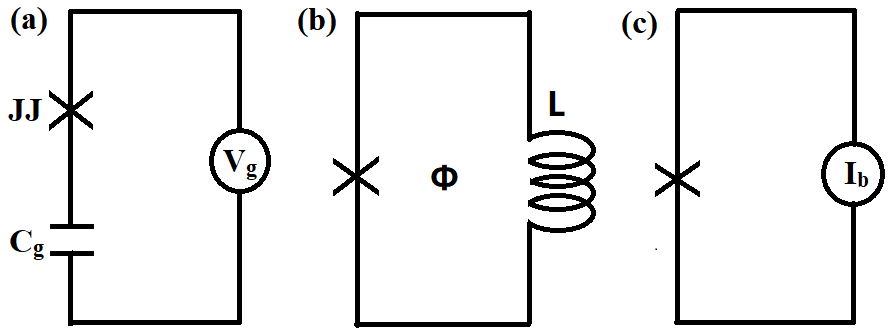
\includegraphics[width=0.8\textwidth]{figures/Superconducting.png}
    \caption{Three types of superconducting qubits circuit diagrams \parencite{Huang_2020}}
    \label{fig:superconducting}
    %referring by label \ref{fig:your-label}.
\end{figure}

\subsection{Photons}
Uses photons as qubits, computations are done via beam splitters, phase shifters, and detectors, that brings several points.

To advantages could be assigned operations with interference and entanglement by room temperatures,
low decoherence due to weak interaction with environment,
could be very helpful in the networks of quantum computers in the future.

Meanwhile, disadvantages include necessity in high-quality hardware to save and detect states,
complex error correction techniques, hard scaling
\parencite{romero2024photonicquantumcomputing}.

\subsection{Topological}
Encodes information non-locally using non-abelian anions such Majorana zero modes in topological superconductors 
or exotic materials. 
Logical gates are implemented via braiding operations that are inherently error-resistant.

Advantages are built-in topological protection that offers resilience to local noise, 
potentially reducing error correction complexity.

Disadvantages are hard experimental realization of stable non-abelian anions,
some operations are still theoretical or nascent.
\parencite{Lahtinen_2017, Zhang_2024}
\subsection{Ion Traps}
Uses positive ions such as Yb or Ca  placed in electromagnetic traps. 
Qubit states are encoded in stable electronic levels.

The strong sites are huge coherence time, that can be exceptionally long also without applying of decoupling techniques,
high fidelity of one-qubit and two-qubit gates, easy state preparation and readout.

The week side is non-triviality by scaling over fifty ions due to heating and crowding.
\parencite{Bruzewicz_2019}
\section{Neutral Atom}
The main considered physical architecture of this paper is \ac{NAQC}. 
This type of computer uses laser cooling and trapping techniques for neutral atoms and
optical or microwave pulses to manipulate quantum states.  
It offers long coherence times, scaling in 2D or even 3D,
and fair connectivities by long-range interactions (Rydberg states).
\subsection{Physical Hardware Implementation}
Consider \ref{fig:ColdAtomArchitecture} to have a schematic overview.
Neutral atoms such as Rubidium, Cesium or Strontium are placed in an ultra-high vacuum cell 
in a specific geometric arrangement often by optical tweezers. 
To work with them, they need to be cooled to very low temperatures.
The process of cooling is multistaged that especially involves Doppler cooling using a laser.
To place cooled atoms on fixed locations and keep them there a trap laser controlled by \ac{SLM} is employed.
With help of \ac{SLM} laser could be focused onto very small configurable points, this effect called optical tweezers.
\ac{SLM} could arrange atoms in 1D, 2D,or even in 3D configuration.
To move atoms there are another mobile traps controlled by \ac{AOD}.
\ac{AOD} implements the similar to \ac{SLM} function, but for mobile optical tweezers.
Then all of these electronic should be precisely calibrated to control process.

To perform actually computations laser and microwaves are employed, 
depends on executed gate used so-called Raman or Rydberg pulses, 
that could work locally or globally on arrangement of neutral atoms. 
\parencite{Schmid_2024_NeutralAtomBasics, Wintersperger_2023}
\begin{figure}[htbp]
  \centering
    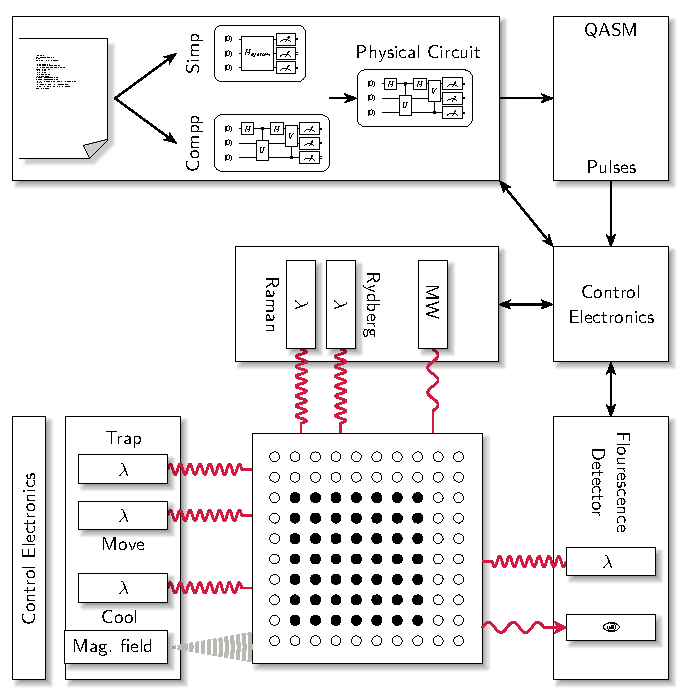
\includegraphics[width=0.8\textwidth]{figures/ColdAtomArchitecture.pdf}
    \caption{Schematic component overview of a cold atom quantum computer \parencite{Wintersperger_2023}}
    \label{fig:ColdAtomArchitecture}
\end{figure}

\subsection{Processing}
To use neutral atoms for performing quantum computations
encoding of qubit computation basis state need be found. 
These encoding should have a long coherence time and weak interaction with environment.
For Rubidium atom it is based on the spin of the furthest electron. 
Meanwhile, a Strontium implementation a nuclear spin of atom is used.

For implementing a one-qubit rotations operators two laser induced so-called Raman transition are used.
Target atom exposure to multiple photons and after that emits some another amount of energy,
what led to change of it state, by combining the duration, power and frequency of laser  
different direction and angles of rotation could be achieved.

For implementing a two-qubit gates a so-called Rydberg state is used. 
In this state an outermost electron has a very huge influence on other atoms' electrons in arrangement.
Thus, other atom cannot go in Rydberg state. This effect called Rydberg blockade.
An effective impact of this effect is a Controlled-Z gate.

Moreover, this effect allows implementing multiple-controlled Z-Gate directly on a hardware,
because Rydberg blockade influences not only on neighbor qubits but as a decreasing by distance field.
The strength of blockade obeys the proportion for small distances \(\frac{1}{|r|^3}\) and \(\frac{1}{|r|^6}\) for long.
Depending on a coefficient that accepted for blocking and interacting, 
different multiple-controlled Z-Gate are implemented.

Also, Rydberg blockade effect is used for long interactions between qubits within the acceptable range, 
it is with \ac{NAQC} possible to execute a two-qubit gate 
and do not require specifically place the atoms directly next to each other.

Nevertheless, if an interaction radius is too small for gate execution,
logical SWAP gates are considered to logically move qubit near to the target qubit.
But \ac{DPQA} could be based on neutral atoms. 
Hence, It makes possible to use physical moving of qubit in lattice, by moving it from \ac{SLM} to \ac{AOD} and back.
This process called shuttling.

For visualization of the described consider \ref{fig:NeutralAtomFeatures}.

\parencite{Wintersperger_2023, Philipp_Wondra_TUM_Thesis_for_Informatics.pdf}

\begin{figure}[htbp]
  \centering
    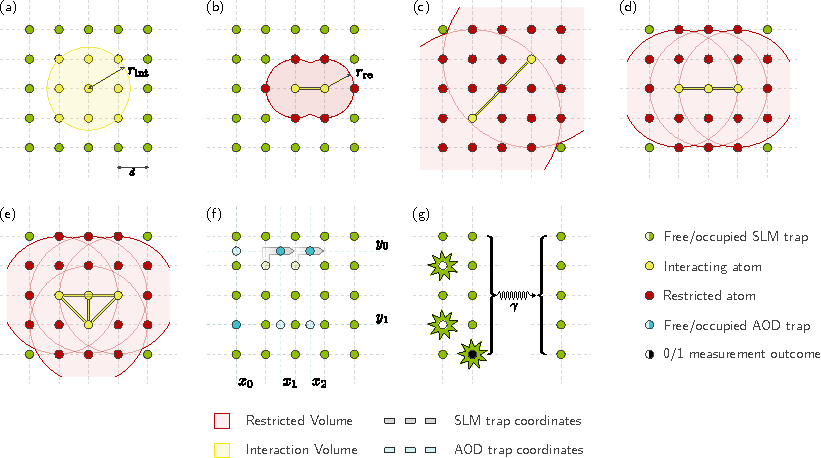
\includegraphics[width=0.8\textwidth]{figures/NeutralAtomFeatures.pdf}
    \caption{\textbf{Capabilities of the NAQC platform.} In this setup, atoms are arranged on a regular grid of \ac{SLM} traps, with a fixed distance denoted as $d$.
  \textbf{(a)} Rydberg blockade interaction: interacting gates can be performed to all qubits within this range.
  \textbf{(b)} Two-qubit gate: A gate can be applied between neighboring qubits but restricts the simultaneous execution of other entangling gates on nearby atoms.
   \textbf{(c)} Long-Range interactions: For gates with larger interaction radii, the restriction zones also expand, resulting in more restricted atoms.
  \textbf{(d)} CCZ gate with a line arrangement of the qubits. 
  According to \cite{Levine_2019} it is sufficient if the central atom interacts with both the outer qubits.
  \textbf{(e)} CCCZ gate 
  \textbf{(f)} Shuttling operation: \ac{AOD} (blue) enable the movement of atoms within the same column or row.
  \textbf{(g)} Additional NA capabilities, useful for future fault-tolerant computations. Not relevant for this work
   \parencite{Schmid_2024_NeutralAtomBasics}.
}\label{fig:NeutralAtomFeatures}
\end{figure}

% !TeX root = ../main.tex
% Add the above to each chapter to make compiling the PDF easier in some editors.

\chapter{Compilation in \ac{NAQC}}\label{chapter:compilation}
Compilation is a process of translating a high-level, 
abstract description of a quantum algorithm into a low-level representation of operations suitable for hardware execution.
To do this, this problem divided into multiple subproblems, 
employing different layers of software each for specific subproblems, so-called compilation toolchain.
Moreover, compilation should be familiar with computational capabilities of target hardware.
As described in \ref{chapter:neutralatom} each compilation step for \ac{NAQC} should consider futher hardware constraints.

For example, that together with or instead of SWAP based losing of connectivity problem
there is also possible to shuttle qubit physical, 
compiler should be able to calculate which way will be the most efficient in terms of speed, fidelity, calculation time in the specific situation.

Hence, compiler should consider different execution times of gates, their fidelities, 
and also an available set of gates on current machine.

Moreover, compiler should consider idle time of qubits and calculate corresponding impact from coherence time.
Thus, it should now which operations could be executed parallel and what properties do \ac{AOD} and \ac{SLM} have.

Also, compiler should consider different interaction radius and Rydberg blockade radius, 
and schedule next step according to constraints that go from previous steps and architecture, 
to improve overall quality of compilation.
\parencite{Tan_2025_Enola,Schmid_2024_NeutralAtomBasics}

\section{Compilation Steps}
Consider \ref{fig:compilation_steps}.
\begin{figure}[htbp]
  \centering
    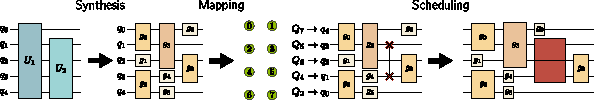
\includegraphics[width=0.8\textwidth]{figures/compilation_steps.pdf}
    \caption{\textbf{Illustration of the three steps for platform-dependent compilation.} In the \textbf{synthesis} step, general operations and unitaries are decomposed into the native gate set $\Sigma_{\mathrm{native}}$.
  During the \textbf{mapping} step, the circuit qubits $q_{i}$ are assigned to physical hardware qubits $Q_{i}$, and necessary SWAP or MOVE operations are introduced to satisfy connectivity constraints.
  Finally, in the \textbf{scheduling} step, gate times and restrictions on parallelism are considered.
  In practice, these steps are often performed simultaneously as a single step rather than sequentially. \parencite{Schmid_2024_NeutralAtomBasics}}
    \label{fig:compilation_steps}
\end{figure}

\section{Considered Toolchains}
In this work three Compiling Toolchains for \ac{NAQC} are considered, 
since they all take a QASM circuit as import and are open-source python projects.
This chapter will cover algorithms that are used by these three, 
describe a workflow, what tools each has, and what consider by compilation
And the result of benchmarking will be evaluated in the next chapter.

\subsection{HybridMapper MQT}
HybridMapper, a Tool from \ac{MQT}, stands out from the previous works, 
because it uses a hybrid compilation approach to map a circuit 
and consider together SWAP gate and Shuttling to explore the potential advantage of leveraging gate-based SWAP insertions 
and shuttling-based atom rearrangements.
When other works individually only considered it separately.
In particular, this is only a mapping and scheduling stage of computation, without synthese and optimization steps.
It simply took a QASM circuit and uses only gates that defined with architecture along with their times, and fidelities 
and doesn't optimize circuit or change something in there, it finds places where interacting conditions are violated 
and solves it with logical or physical move. 
In advance, skipping synthese step gives advantages, 
since other considered toolsets always try to transpile input circuit into Pauli Gates and CZ gate, without consideration of possible multi-qubit CZ gates.

The main idea of algorithm is to use two-capability-specific heuristic cost functions, 
which specially made for fast evaluation 
and consider additional architecture information 
such as number of \ac{AOD} or \ac{SLM} traps, distance between them, interaction radius 
to improve parallelism by using commutation rules and look-ahead functionality \parencite{schmid2023hybridcircuitmappingleveraging}.
Consider for accuracy \ref{fig:overview_HybridMapper}.

\begin{figure}[htbp]
  \centering
    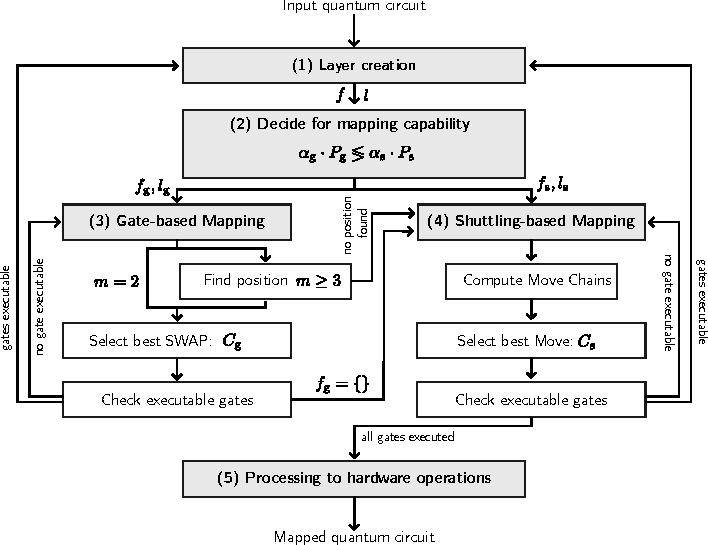
\includegraphics[width=0.8\textwidth]{figures/overviewHybridMapper.pdf}
    \caption{Resulting hybrid mapping process \parencite{schmid2023hybridcircuitmappingleveraging}}
    \label{fig:overview_HybridMapper}
\end{figure}
\subsection{Enola}
Enola a Tool from \ac{UCLA-VAST} based on OLSQ-DPQA uses different approach.
It divides mapping and scheduling steps of compilation into scheduling, placement and routing steps to achieve great fidelity.

Scheduling step is implemented thorough Edge Coloring problem of commutation group (a group consisting of commutable two-qubit
gates that can be executed in any order) graph, 
where vertices are qubits and edges are two-qubit gates. 
This problem then is solved using Misra-Gries algorithm.
For more generic circuits Enola can use the dependency DAG (directed acyclic graph) for the two-qubit
gates in a generic circuit. In this case, the scheduling problem is
straightforward: the optimal number of stages is the critical path
in the DAG and ASAP (as soon as possible) scheduling can achieve
optimality \parencite{Tan_2025_Enola}a. Visualization \ref{fig:scheduling_Enola}
\begin{figure}[htbp]
  \centering
    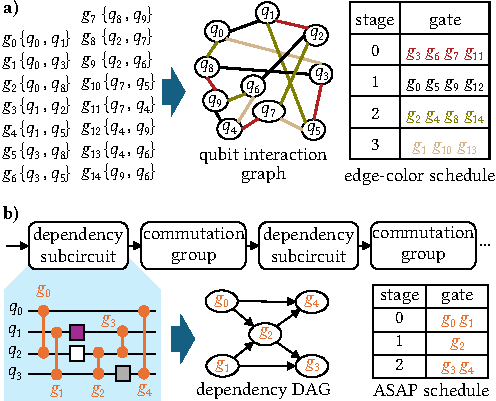
\includegraphics[width=0.8\textwidth]{figures/scheduling_Enola.pdf}
    \caption{ Scheduling in Enola. 
    \textbf{(a)} Scheduling a commutation group of two-qubit gates with edge coloring. 
    \textbf{(b)} Generic circuits can be divided to dependency subcircuits and commutation groups. 
    Dependency subcircuits are scheduled ASAP \parencite{Tan_2025_Enola}.}
    \label{fig:scheduling_Enola}
\end{figure}

Placement step is implemented through fast simulated annealing, 
qubits are mapped to interaction sited and the two-qubit
gates at each Rydberg stage are like 2-pin nets in conventional
circuit placement. Hence, the goal is ti minimize total "wire-length".
Fast simulated annealing has three-stages to explore possible states.
At the first stage random search to explore a large solution space is used, the temperature is high, 
thus a high probability of bad solution.
Then, the second stage is a pseudo-greedy local search. 
The last stage is a hill-climbing search where
the temperature increases again to escape from local minima \parencite{Tan_2025_Enola}. 
Visualization \ref{fig:placement_Enola}.
\begin{figure}[htbp]
  \centering
    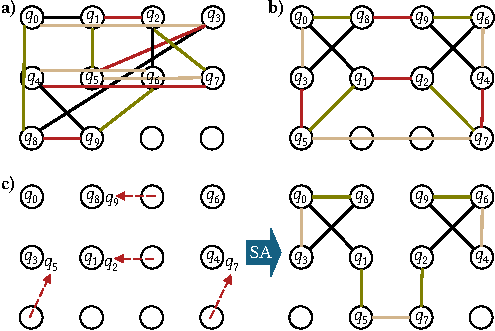
\includegraphics[width=0.8\textwidth]{figures/placement_Enola.pdf}
    \caption{ Placement in Enola. 
    \textbf{(a)} Trivial placement from left to right, from top to bottom. 
    \textbf{(b)} Placement with gate distance optimized by simulated annealing. 
    \textbf{(c)} Dynamic placement: after a Rydberg stage (red) is executed (left), run simulated
    annealing on moved qubits for a new placement (right). \parencite{Tan_2025_Enola}}
    \label{fig:placement_Enola}
\end{figure}

Routing step is used for parallelize \ac{AOD} movements, 
and not to violate fundamental rules of \ac{AOD} such as \textit{the order of its columns cannot change, nor can
the order of rows}.
Then the independent set of vertices is made of possible moves. 
This set will be solved then with maximum independent set solver \parencite{Tan_2025_Enola}.
Visualization \ref{fig:routing_Enola}.
\begin{figure}[htbp]
  \centering
    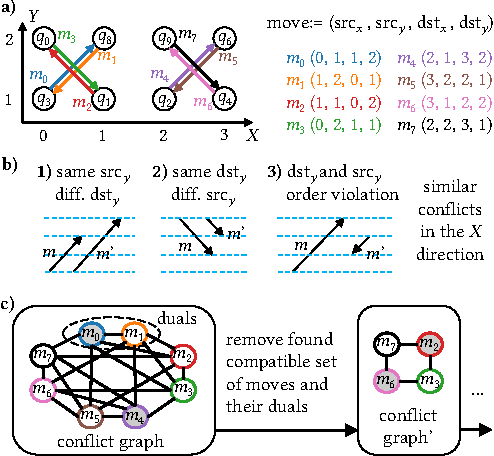
\includegraphics[width=0.8\textwidth]{figures/routing_Enola.pdf}
    \caption{Routing in Enola. 
    \textbf{(a)} Definition of a move as a 4-tuple. 
    \textbf{(b)} Conflicts between two moves. 
    \textbf{(c)} Compatible moves are independent sets (IS) in the conflict graph (filled vertices).
    After finding an IS, delete the moves and their duals from
    the graph. The process continues until no moves are left \parencite{Tan_2025_Enola}.}
    \label{fig:routing_Enola}
\end{figure}

Additionally, Enola always transpiles input circuit into fixed gate set from Pauli Gates and CZ, 
without consideration of a big advantage of \ac{NAQC} that allows to implement different gates.
Also, it considers interaction radius, Rydberg blockade radius, durations and fidelities of gates,
physical placement of \ac{SLM} and \ac{AOD} traps. 
But important note is that Enola doesn't consider number of \ac{AOD}, 
but make an independent set of gates called stages where each pair of gates could be executed without affecting other qubits in that stage.

\subsection{DasAtom}
DasAtom was made as an improvement of Enola and Tetris 
and used the weakest aspects of each to strengthen and made itself.
Enola leverages atom shuttling to adapt qubit mappings dynamically,
but cannot take advantage of long-range interactions
and Tetris' main idea is to leverage the long-range interactions of \ac{NAQC} 
to achieve denser qubit connectivity\parencite{10082942, huang2025dasatomdivideandshuttleatomapproach}.

The main idea of DasAtom is a bit changed \ac{DAC} approach to divide circuit into subcircuits.
It was inspired from different DAC adaptations from \parencite{siraichi:hal-02316820, 10.1145/3508352.3549394, huang2024qubitmappingadaptivedivideandconquer}
Then it assigns an optimal qubit mapping for each subcircuit, and then shuttles
atoms to smoothly transition between mappings. This approach should improve overall fidelity and efficiency.
Consider \ref{fig:DasAtomFlowChart}

\begin{figure}
\centering
\scalebox{0.78}{
\begin{tikzpicture}[node distance=1.5cm]

% Nodes
\node (start) [startstop] {Input: CZ circuit $C$, $d$, $R_{\mathrm{int}}$, $R_{\mathrm{restr}}$};
\node (partition1) [process, below of=start] {Divide $C$ into CZ layers $L_1,...L_m$};
\node (partition2) [process, below of=partition1] {Divide $C$ into $C_1, ..., C_k$ and find an embedding $f_i$ for each $C_i$};
%\node (init) [process, below of=partition2] {Let $i = 1$};
\node (execute) [process, below of=partition2] {Start with $i=1$ and execute $C_i$ with $f_i$};
\node (decision) [decision, below of=execute, yshift=-0.5cm] {$i = k?$};
\node (route) [process, below of=decision, yshift=-0.5cm] {Route $f_i$ to $f_{i+1}$};
\node (increment) [process, left of=route, xshift=-2.5cm] {$i = i + 1$};
\node (end) [startstop, right of=decision, xshift=1.5cm] {End};
% Arrows
\draw [arrow] (start) -- (partition1);
\draw [arrow] (partition1) -- (partition2);
\draw [arrow] (partition2) -- (execute);
\draw [arrow] (execute) -- (decision);
\draw [arrow] (decision) -- node[anchor=east] {no} (route);
\draw [arrow] (route) -- (increment);
\draw [arrow] (increment) |- (execute.west);
\draw [arrow] (decision) -- node[anchor=south] {yes} (end);

\end{tikzpicture}}
\caption{The flowchart of DasAtom \parencite{huang2025dasatomdivideandshuttleatomapproach}.}
\label{fig:DasAtomFlowChart}
\end{figure}

DasAtom states about 415.8 times higher fidelity comparing to Enola in \ac{QFT}30. 
This statement doesn’t quite seem to be full correct.
\parencite{huang2025dasatomdivideandshuttleatomapproach}
% !TeX root = ../main.tex
% Add the above to each chapter to make compiling the PDF easier in some editors.

\chapter{Evaluation}\label{chapter:evaluation}
\parencite{Emil_Khusainov_Bachelor_GIT}
\subsection{HybridMapper \ac{MQT}}
\subsection{Enola}
\subsection{DasAtom}
% !TeX root = ../main.tex
% Add the above to each chapter to make compiling the PDF easier in some editors.

\chapter{Conclusion And Outlook}\label{chapter:conclusion}
\section{Conclusion}
\ac{NAQC} represent a new hardware architecture with exclusive combination of capability and constraints.
This architecture has huge perspectives in world of quantum computations. 
Nevertheless, to subjugate all the power of it a good software solution must be produced.

This work was focused on benchmarking of existing compilation toolchains 
and the most important thing is an honest comparison. What was fullified in this paper.

Firstly, a test setup was created, to bring all tool chains into similar conditions, and first testing was performed.

Secondly, results were interpreted, and suspicious things were investigates and repaired.

Thirdly, the new testing was performed, that has shown a worthy results 
such as finding that difference is actually not a 400x times and exponential grow as DasAtom \parencite{huang2025dasatomdivideandshuttleatomapproach} states, 
but either 5.5x times between Enola and DasAtom. 
\section{Outlook}
As a result, some further work could be done. Something such as adding new compiler toolchains for comparison.
Or something deeper, 
such as consideration of all possible parameters that take place for example in Enola but don't in other,
and due to not very big impact on calculations, often it is not being considered.
Moreover, different circuits could be used, with different level of start optimizations to see actually performance of a tool chain.
% TODO: add more chapters here

\appendix{}

\microtypesetup{protrusion=false}

\addchap{Abbreviations}
\begin{acronym}
	\itemsep-.25\baselineskip
	\acro{TUM}[TUM]{Technical University of Munich}
	\acro{DPQA}[DPQA]{Dynamically Field-Programmable Qubit Arrays}
	\acro{NAQC}[NAQC]{Neutral Atom Quantum Computer}
	\acro{QC}[QC]{Quantum Computer}
	\acro{NISQ}[NISQ]{Noisy Intermediate Scale Quantum Computing Era}
	\acro{FTQC}[FTQC]{Fault-Tolerant Quantum Computing Era}
	\acro{SLM}[SLM]{Spatial Light Modulator}
	\acro{AOD}[AOD]{Acousto-Optic Deflector}
	\acro{MQT}[MQT]{Munich Quantum Valey}
	\acro{UCLA-VAST}[UCLA-VAST]{UCLA-VAST Lab}
	\acro{QFT}[QFT]{Quantum Fourier transform}
	\acro{DAC}[DAC]{Divide-and-conquer}
	\acro{HM}[HM]{HybridMapper}
	% TODO: add acronyms
\end{acronym}

\listoffigures{}
\listoftables{}
\microtypesetup{protrusion=true}
\printbibliography{}

\end{document}
